%%%%%%%%%%%%%%%%%%%%%%%%%%%%%%%%%%%%%%%%%
% Structured General Purpose Assignment
% LaTeX Template
%
% This template has been downloaded from:
% http://www.latextemplates.com
%
% Original author:
% Ted Pavlic (http://www.tedpavlic.com)
%
% Note:
% The \lipsum[#] commands throughout this template generate dummy text
% to fill the template out. These commands should all be removed when
% writing assignment content.
%
%%%%%%%%%%%%%%%%%%%%%%%%%%%%%%%%%%%%%%%%%

%	PACKAGES AND OTHER DOCUMENT CONFIGURATIONS

\documentclass[a4paper]{article}
\usepackage[utf8]{inputenc}
\usepackage[T1]{fontenc}
\usepackage[english]{babel}
\usepackage{fancyhdr} % Required for custom headers
\usepackage{lastpage} % Required to determine the last page for the footer
\usepackage{extramarks} % Required for headers and footers
\usepackage{graphicx} % Required to insert images
\usepackage{amsmath,amssymb,amsthm,amsfonts}
\usepackage{cleveref}
\usepackage{pdfpages}
\usepackage{float}


\usepackage{listings}
\usepackage{color} %red, green, blue, yellow, cyan, magenta, black, white
\definecolor{mygreen}{RGB}{28,172,0} % color values Red, Green, Blue
\definecolor{mylilas}{RGB}{170,55,241}

% Margins
\topmargin=-0.45in
\evensidemargin=0in
\oddsidemargin=0in
\textwidth=6.3in
\textheight=9.6in
\headsep=0.25in

\linespread{1.1} % Line spacing

% Set up the header and footer
\pagestyle{fancy}
\lhead{\hmwkAuthorName} % Top left header
\chead{\hmwkTitle} % Top center header
\rhead{\hmwkClass} % Top right header
\lfoot{} % Bottom left footer
\cfoot{} % Bottom center footer
\rfoot{Page\ \thepage\ of\ \pageref{LastPage}} % Bottom right footer

\renewcommand\headrulewidth{0.4pt} % Size of the header rule
\renewcommand\footrulewidth{0.4pt} % Size of the footer rule

\setlength\parindent{0pt} % Removes all indentation from paragraphs

\setcounter{secnumdepth}{0} % Removes default section numbers

%	NAME AND CLASS SECTION

\newcommand{\hmwkTitle}{Classical Loop-Shaping} % Assignment title
\newcommand{\hmwkClass}{EL2520} % Course/class
\newcommand{\hmwkClassName}{Control Theory and Practice} % Course/class
\newcommand{\hmwkAuthorName}{Stiernman, Bhustalimath} % Your name

%	TITLE PAGE

\title{
	\vspace{1.5in}
	\textmd{\textbf{\hmwkClass\ -- \hmwkClassName}}\\
	\vspace{0.2in}
	\textmd{\textbf{\hmwkTitle}}\\
	\normalsize\vspace{0.1in}\small{\today}\\
	\vspace{2in}
}
\author{
	Karl Stiernman\\
	ksti@kth.se\\
    920301-6010
	\and
	Sangharsh Bhustalimath\\
	sbhu@kth.se\\
	940419-8252
}
\date{}

%%%%%%%%%%%%%%%%%%%%%%%%%%%%%%%%%%%%%%%%%%%%%%%%%%

\begin{document}

\maketitle

\vfill
\begin{abstract}
	The report consists of the application of Classical Loop-shaping technique in the design of controllers, initially without the consideration of disturbances, and later, with the consideration of a disturbance model and the attenuation of it.
\end{abstract}
%it's attenuation in the system.
\newpage


%%%%%%%%%%%%%%%%%%%%%%%%%%%%%%%%%%%%%%%%%%%%%%%%%%


\lstset{language=Matlab,%
    %basicstyle=\color{red},
    breaklines=true,%
    morekeywords={matlab2tikz},
    keywordstyle=\color{blue},%
    morekeywords=[2]{1}, keywordstyle=[2]{\color{black}},
    identifierstyle=\color{black},%
    stringstyle=\color{mylilas},
    commentstyle=\color{mygreen},%
    showstringspaces=false,%without this there will be a symbol in the places where there is a space
    numbers=left,%
    numberstyle={\tiny \color{black}},% size of the numbers
    numbersep=9pt, % this defines how far the numbers are from the text
    emph=[1]{for,end,break},emphstyle=[1]\color{red}, %some words to emphasise
    %emph=[2]{word1,word2}, emphstyle=[2]{style},    
}

%%%%%%%%%%%%%%%%%%%%%%%%%%%%%%%%%%%%%%%%%%%%%%%%%%%%%%
\section{Basics}
A lead-lag compensator $F$ was designed for the system given in \cite{exercise} modeled by the following transfer function:
\begin{equation}
	G(s) = \frac{3(-s+1)}{(5s+1)(10s+1)}.
	\label{eq:system}
\end{equation}

The lead-lag compensator was designed such that the closed-loop system  given in \cref{fig:block_diagram} fulfills the following specifications:
\begin{itemize}\setlength{\itemsep}{-2pt}
	\item Crossover frequency $\omega_c = 0.4$ rad/s.
	\item Phase margin $\phi_m = 30^\circ$.
	\item Zero stationary error for step response. 
    % I have put error as 2% here because that is the error I am getting from the code
\end{itemize}

\begin{figure}[!ht]
	\begin{center}
		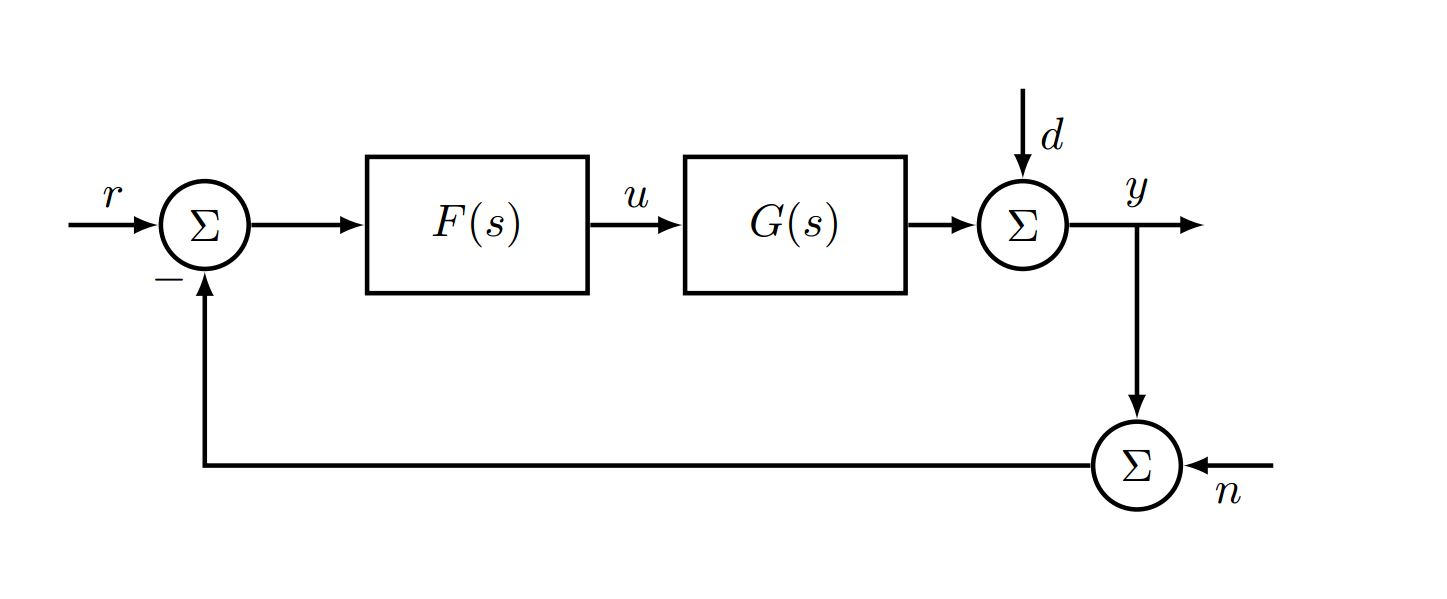
\includegraphics[width=0.5\textwidth]{system}
	\end{center}
	\caption{Closed-loop block diagram, where $F$--controller, $G$--system, $r$--reference signal, $u$--control signal, $d$--disturbance signal, $y$--output signal, $n$--measurement noise.}
	\label{fig:block_diagram}
\end{figure}

The procedure given in \cite{basic_book} was used to determine the parameters $K, \beta, \tau_D, \tau_i, \gamma$ of the lead-lag compensator:
\begin{equation}
	F(s) = K \frac{\tau_D s + 1}{\beta \tau_D s + 1} \frac{\tau_I s + 1}{\tau_I s + \gamma}.
	\label{eq:lead_lag}
\end{equation}
The system's phase, $\arg(G(i\omega_c)) = 161.2^\circ$, was determined from the Bode diagram in \cref{fig:bode_diagram}. Initially, the compensator was designed to have a phase margin of $30^\circ$ and it was found out that an excess of 5.9$^\circ$ had to be added to account for the lag part.

\begin{figure}[!ht]
	\begin{center}
		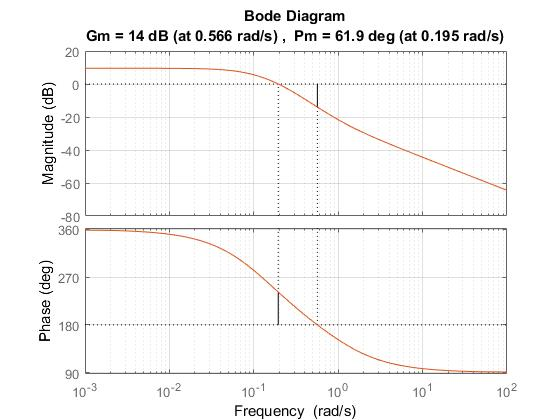
\includegraphics[width=.8\linewidth]{bodeG}
	\end{center}
	\caption{Bode diagram for system $G(s)$ in \eqref{eq:system}.}
	\label{fig:bode_diagram}
\end{figure}

Thus, the necessary phase shift was:
\[
	30^\circ - (180^\circ-161.2^\circ) + 5.9^\circ = 11.2^\circ + 5.9^\circ = 17.1^\circ
\]

The first parameter $\beta$ was evaluated from \cref{eq:beta} from \cite{basic_book}.
\begin{equation}
\phi_{max}=\arctan(\frac{1-\beta}{2\sqrt\beta}).
\label{eq:beta}
\end{equation}

Parameter $\tau_D$ was evaluated using \cref{eq:taud}:
\begin{equation}
\tau_D=\frac{1}{\omega_c\sqrt\beta}.
\label{eq:taud}
\end{equation}
Parameter $K$ was evaluated using \Cref{eq:k}:
\begin{equation}
K=\frac{1}{\lvert F_{lead}(i\omega_c)G(i\omega_c)\lvert}.
\label{eq:k}
\end{equation}
The parameter $\gamma$ was picked to cancel the steady state error while making sure that $F_{lead}$ is stable. The value for $\tau_I$ was chosen according to \cref{eq:taui}:
\begin{equation}
\tau_I=\frac{10}{\omega_c}
\label{eq:taui}
\end{equation}

The final controller, given by \cref{eq:lead_lag} has the parameters given in \cref{tb:lead_lag_parameters}.

\begin{table}[!ht]
\begin{center}
	\begin{tabular}{|c|c|c|c|c|}
		\hline
		$K$ & $\beta$ & $\tau_D$ & $\tau_i$ & $\gamma$\\
		\hline
		2.1075 & 0.5455 & 3.3847 & 25.0000 & 0\\
		\hline
	\end{tabular}
\end{center}
\caption{Parameters for the lead-lag compensator.}
\label{tb:lead_lag_parameters}
\end{table}

The bandwidth ($\omega_B$) and resonance peak ($M_T$) of the closed-loop system was determined from its bode plot in \cref{fig:bode_closedloop}.

\begin{figure}[!ht]
\centering
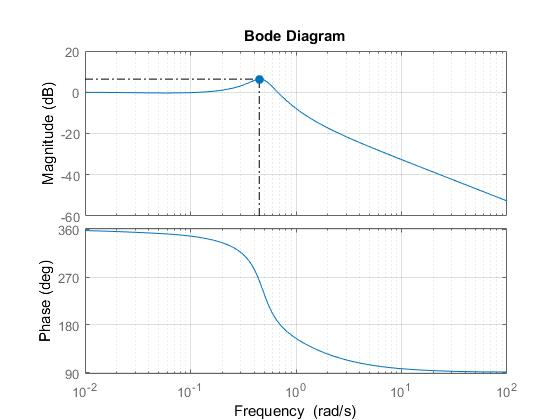
\includegraphics[width=.8\linewidth]{bode_closedloop}
\caption{Bode plot for the closed-loop system in \cref{fig:block_diagram}, with the lead-lag compensator.}
\label{fig:bode_closedloop}
\end{figure}

The rise time ($T_r$) and overshoot ($M$) was determined form the step response in \cref{fig:step_response}, and given in \cref{tb:response}.

\begin{figure}[!ht]
	\begin{center}
		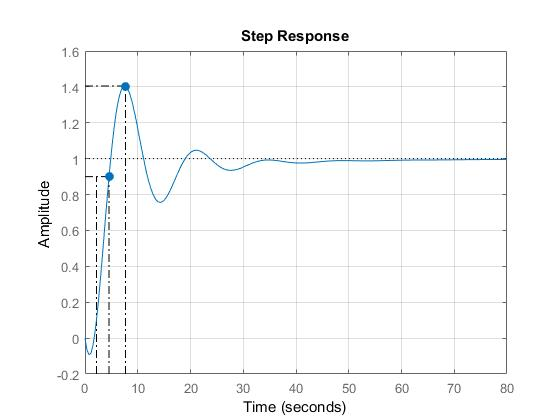
\includegraphics[width=.75\linewidth]{step_response}
	\end{center}
	\caption{Step response for the closed-loop system in \cref{fig:block_diagram}, with the lead-lag compensator.}
	\label{fig:step_response}
\end{figure}

\begin{table}[!h]
\begin{center}
	\begin{tabular}{|c|c|c|c|}
		\hline
		$\omega_B$ [rad/s] & $M_T$ [dB] & $T_r$ [s] & $M$ [\%] \\
		\hline
		0.77 & 6.36 & 2.39 & 40.00 \\
		\hline
	\end{tabular}
\end{center}
\caption{Closed loop system characteristics.}
\label{tb:response}
\end{table}

The controller was now modified to obtain a phase margin of $\phi=50^\circ$ while maintaining the same cross over frequency of $\omega_c=.4$, by evaluating the necessary phase margin: 

\[50^\circ-(198.7-180)+5.9 = 37.2 \]

An excess of $5.9^\circ$ was added to account for the lag part. The Open-loop bode plot of the system with the modified controller is as seen in \cref{fig:bode_openloop_ph50}.

\begin{figure}[!ht]
\centering
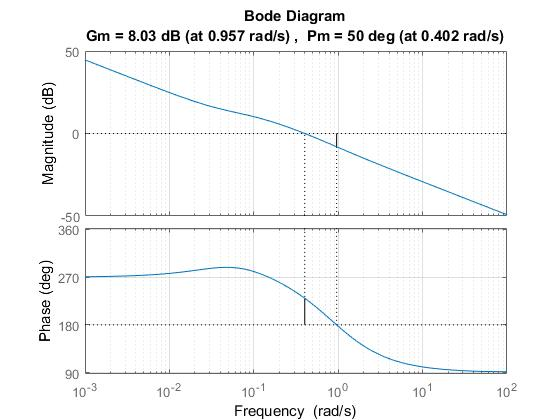
\includegraphics[width=.8\linewidth]{bode_openloop_ph50_n}
\caption{Open loop Bode plot for the system given in \cref{fig:block_diagram} with the modified controller}
\label{fig:bode_openloop_ph50}
\end{figure}

%% bandwith and resonance peak for system 50 ph 
The bandwidth ($\omega_{B2}$) and resonance peak ($M_{T2}$) of the new closed-loop system was determined from its bode plot in \cref{fig:bode_closedloop_ph50}

\begin{figure}[!ht]
\centering
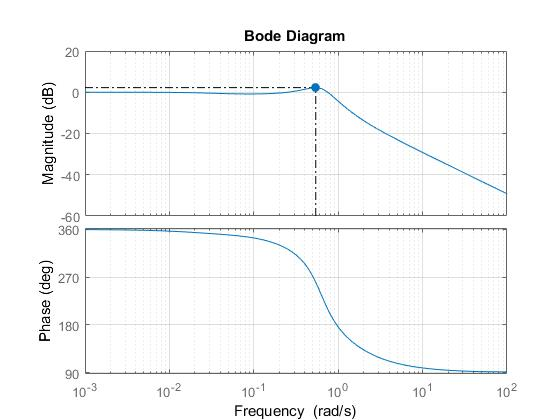
\includegraphics[width=.8\linewidth]{bode_closedloop_ph50}
\caption{Bode Plot for the closed loop system in \cref{fig:block_diagram}, with the modified lead-lag compensator}
\label{fig:bode_closedloop_ph50}
\end{figure}

%% rise time ,, overshoot for system 50 ph 
The rise time ($T_{r2}$) and overshoot ($M_2$) of the new system was determined form the step response in \cref{fig:step_response_ph50}, and given in \cref{tb:response_ph50}.

\begin{figure}[!ht]
	\begin{center}
		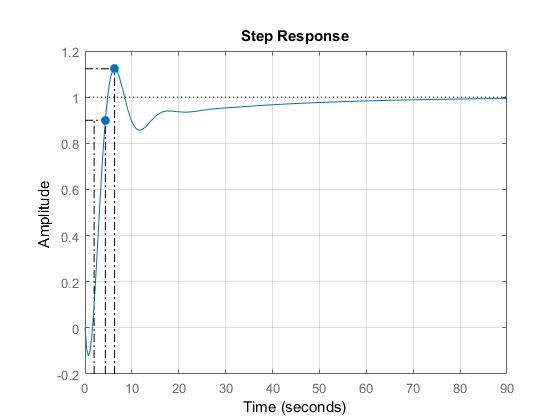
\includegraphics[width=.8\linewidth]{step_response_ph50}
	\end{center}
	\caption{Step response for the closed loop system in \cref{fig:block_diagram}, with the modified lead-lag compensator.}
	\label{fig:step_response_ph50}
\end{figure}

%% Closed loop system characteristics
\begin{table}[!ht]
\begin{center}
	\begin{tabular}{|c|c|c|c|}
		\hline
		$\omega_{B2}$ [rad/s] & $M_{T2}$ [dB] & $T_{r2}$ [s] & $M_2$ [\%] \\
		\hline
		 0.92 & 2.25 & 2.41 & 12.30 \\
		\hline
	\end{tabular}
\end{center}
\caption{Closed loop system characteristics of the system with modified controller.}
\label{tb:response_ph50}
\end{table}

\section{Disturbance attenuation}

%% 4.2.1
In this section a disturbance transfer function $G_d(s)$  which is modeled as shown in \cref{eq:dist} and a prefilter function $F_r(s)$ is considered as shown in the System Block Diagram in \cref{fig:block_dist}.

\begin{equation}
G_d(s) = \frac{10}{s+1}
\label{eq:dist}
\end{equation}

\begin{figure}[H]
	\begin{center}
		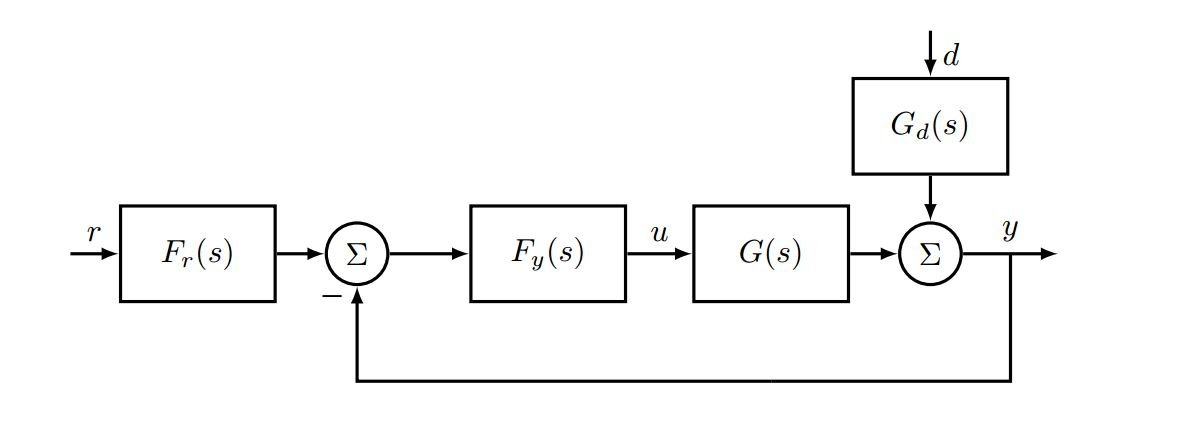
\includegraphics[width=0.5\textwidth]{system_dist}
	\end{center}
	\caption{Closed loop block diagram, where $F_r$--prefilter, $F_y$--controller, $G$--system, $G_d$--disturbance dynamics, $r$--reference signal, $u$--control signal, $d$--disturbance signal, $y$--measurement signal, $n$--measurement noise.}
	\label{fig:block_dist}
\end{figure}

For the disturbances to be attenuated, the control action was required at all the frequencies where $\lvert G_d(s)\lvert >1$. The crossover frequency ($\omega_{cd}$) for the disturbance model in \cref{eq:dist} was obtained from it's bode plot in \cref{fig:bode_gd}.

\begin{figure}[!ht]
\centering
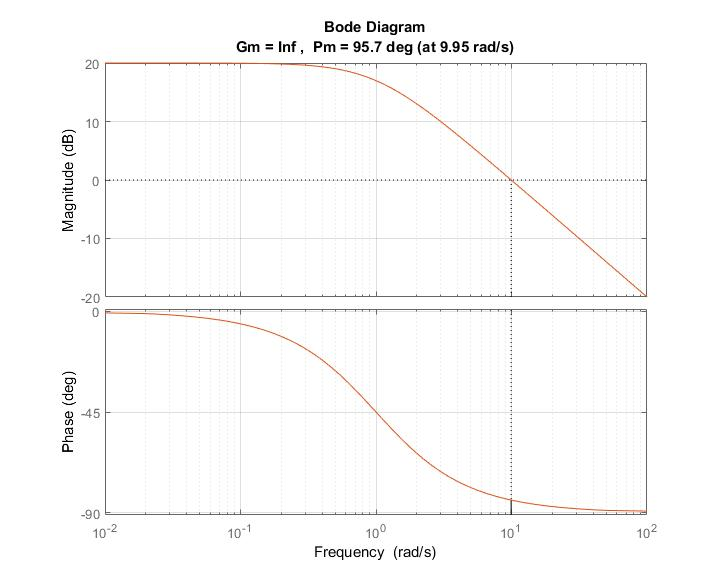
\includegraphics[width=.8\linewidth]{bode_gd}
\caption{Bode plot of the transfer function in \cref{eq:dist}}
\label{fig:bode_gd}
\end{figure}

The controller ($F_y$) was designed according to \cref{eq:contrimproper}, but this controller was improper and has an order of two in the numerator and zero in the denominator, so two poles need to be added to make this transfer function proper. 

\begin{equation}
F_y=G^{-1}\omega_c/s
\label{eq:contrimproper}
\end{equation}

The poles need to be added such that the controller's gain behavior for all frequencies where the disturbance needs to be attenuated (i.e. for all frequencies where $\lvert G_d(i\omega)\lvert>1$) stays the same before and after the introduction of the two poles. The two poles were introduced at -80 as shown in \cref{eq:contrproper}. It can be seen that the controller's gain behavior for the proper and improper forms,for all frequencies where $\lvert G_d(i\omega)\lvert>1$, stays the same after the addition of the two poles as shown in \cref{fig:gain_behavior}. 

\begin{equation}
F_y=G^{-1}\frac{\omega_c}{s}\frac{1}{(s/80+1)^2}
\label{eq:contrproper}
\end{equation}


\begin{figure}[!ht]
\centering
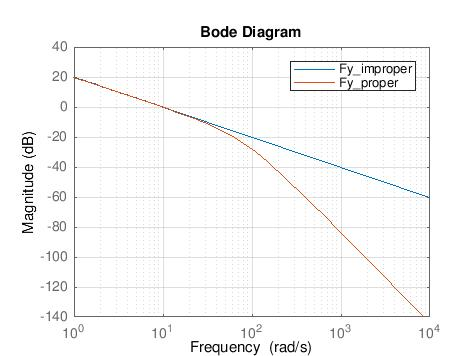
\includegraphics[width=.8\linewidth]{bodemag_421}
\caption{Comparison of Gains of the controller ($F_y$) before and after addition of the two poles at -80}
\label{fig:gain_behavior}
\end{figure}

It was observed that an integral action was needed for the disturbance attenuation at frequencies where $\lvert G_d\lvert>1$, so the controller $F_y$ was chosen as a PI controller according to \cref{eq:PIaction}. The parameter $\omega_I=10$ was chosen because efficient integral action is needed at frequencies between 0 rad/s and $\omega_{cd}=9.95$ rad/s.

\begin{equation}
F_y=\frac{s+\omega_I}{s}G^{-1}G_d
\label{eq:PIaction}
\end{equation}

A low pass filter with the transfer function $F_r$ as shown in \cref{eq:filter}, was added to the reference signal to fulfill reference tracking conditions. The parameter $\tau$ in \cref{eq:PIaction} was chosen to be equal to 1. The filter $F_r$ has to be simple because it is the signal that the controller tracks, thus to track a complicated reference signal, one would require an even more complicated controller. 

\begin{equation}
F_r=\frac{1}{1+\tau s}
\label{eq:filter}
\end{equation}

The response of the output ($y$) was observed with respect to step inputs in the reference signal ($r$), as shown in \cref{fig:stepresponse_ytor}, and the disturbance signal ($d$) as shown in \cref{fig:stepresponse_ytod}, according to \cref{eq:y}.

\begin{figure}[!ht]
\centering
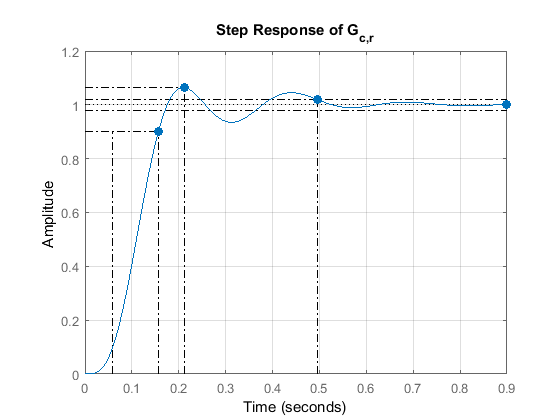
\includegraphics[width=.8\linewidth]{Gcr_423}
\caption{Step response of the closed-loop system from the reference signal to the output. Rise time 0.0973 s; overshoot $M=6.43$ \%.}
\label{fig:stepresponse_ytor}
\end{figure}

\begin{figure}[!ht]
\centering
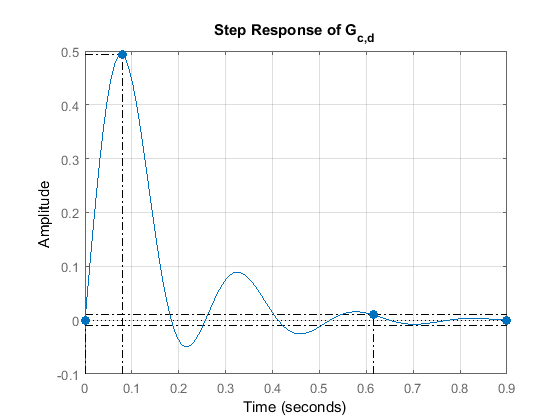
\includegraphics[width=.8\linewidth]{Gcd_423}
\caption{Step response of the closed-loop system from the disturbance signal to the output. The response goes to zero for increasing time, with peak amplitude 0.493 and the highest amplitude after $t=5$ s is equal to 0.0156.}
\label{fig:stepresponse_ytod}
\end{figure}

\begin{equation}
y=SG_dd + TF_rr
\label{eq:y}
\end{equation}

$S$ and $T$ in \cref{eq:y} are sensitivity and complementary sensitivity functions given by \cref{eq:s} and \cref{eq:t} respectively.

\begin{equation}
S=\frac{1}{1+GF_y}
\label{eq:s}
\end{equation}

\begin{equation}
T=\frac{GF_y}{1+GF_y}
\label{eq:t}
\end{equation}

The size of the control signal $u$ was observed with respect to th step inputs in the reference signal ($r$), as shown in \cref{fig:stepresponse_utor}, and the disturbance signal ($d$) as shown in \cref{fig:stepresponse_utod}, according to \cref{eq:u}. In doing this, the signals $r$ and $d$ were considered independently, i.e. the step response from $r$ to $u$ was studied considering $d=0$ and vice versa. 

\begin{figure}[!ht]
\centering
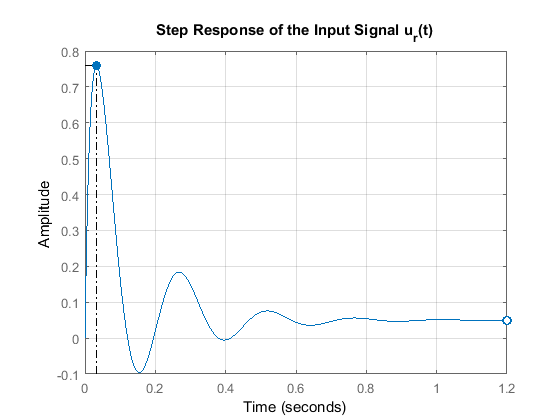
\includegraphics[width=.8\linewidth]{ur_423}
\caption{Response of the input signal ($u$) to a step input in $r$. The peak amplitude is 0.863.}
\label{fig:stepresponse_utor}
\end{figure}

\begin{figure}[!ht]
\centering
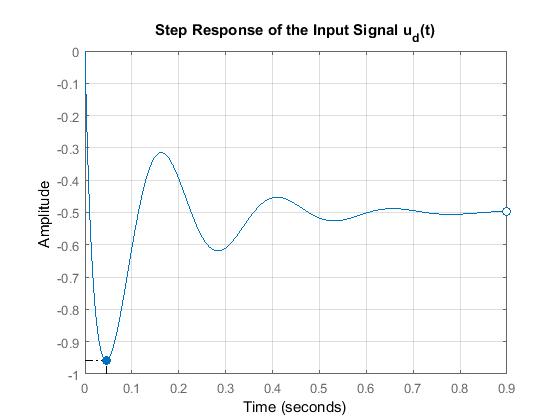
\includegraphics[width=.8\linewidth]{ud_423}
\caption{Response of the input signal ($u$) for a step input in $d$. The peak amplitude is -0.958.}
\label{fig:stepresponse_utod}
\end{figure}

\begin{equation}
u=F_yF_rSr - F_yG_dSd
\label{eq:u}
\end{equation}

It can be seen from the figures \cref{fig:stepresponse_utor} and \cref{fig:stepresponse_utod} that the input signal will be guaranteed to be less than 1 for all $r$ and $d$ scaled on the interval $[0,1]$.

A lead compensator ($F_{lead}$) was added to the controller to reduce the overshoot of y with respect to the reference signal, according to \cref{eq:lead}. On tuning the parameters $\beta$ and $\tau_D$ were found to be 0.33 and ... respectively.

\begin{equation}
F_{lead}=\frac{\tau_Ds+1}{\beta\tau_Ds_1}
\label{eq:lead}
\end{equation}

\begin{figure}[!ht]
\centering
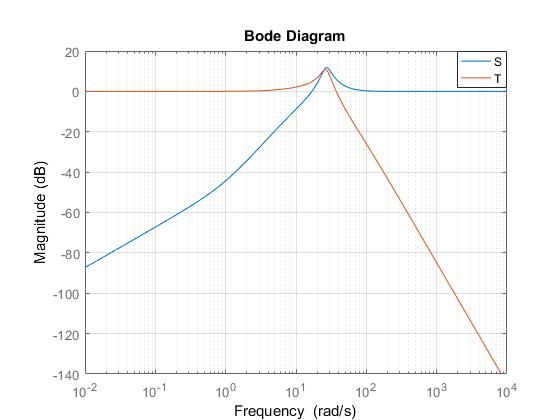
\includegraphics[width=.8\linewidth]{ST}
\caption{Bode Plot of Sensitivity ($S$) and Complementary Sensitivity ($T$)}
\label{fig:st}
\end{figure}
\section{Conclusions}
The output ($y$) of the system shown in \cref{fig:block_dist} is expressed as a function of sensitivity ($S$) and complementary sensitivity ($T$) in \cref{eq:y}. 
The disturbances ($d$), that belong to a given low frequency band in such a system, can be attenuated by manipulating the sensitivity, but at the same time this affects the tracking of the reference signal. This is due to the fact that the sum of sensitivity and complementary sensitivity has to be unity. A trade-off is thus made, at the expense of rise time, to suppress the overshoot of the output due to the reference signal by adding a Lead compensator.

A controller can hence, be designed by making a trade-off between the frequency bandwidths of disturbance and noise, such that the disturbance is attenuated at lower frequencies and the measurement noise at higher frequencies, as can be seen from \cref{fig:st}.
\\ \\
\newpage

\begin{thebibliography}{9}

\bibitem{exercise}
EL2520 Control Theory and Practice Advanced Course, \emph{Computer Exercise: Classical Loop-Shaping}, 2014.

\bibitem{basic_book}
T. Glad and L. Ljung, \emph{Reglerteknik, Grundläggande teori}, Studentlitteratur, 2006.

\end{thebibliography}


%%%%%%%%%%%%%%%%%%%%%%%%%%%%%%%%%%%%%%%%%%%%%%%%%%


%\newpage
%\section{Appendix A: Matlab code}
%\includepdf[pages={1-2}]{Example.pdf}
%\lstinputlisting{lab1_team.m}


%\newpage
%\section{Some reminders}
%\begin{itemize}
%	\item Write clear and concise, but comprehensible. No novels!
%	\item The report should be self-contained, don't assume the reader %knows the lab instructions.
%	\item However, don't repeat material from the course book, instead, use references.
%	\item Make sure that all results and figures are reproducible.
%	\item Start with a \emph{short} summary of the results and the contents of the report.
%	\item Motivate all the choices you have done.
%	\item Show results in tables and figures that are easy to compare.
%	\item Introduce figures in the text where it is needed, and remember to describe what the figure shows, what the axes corresponds to and what the results are.
%	\item Be specific in your writing, and avoid vague expressions such as ``some'' and ``not so good''.
%	\item Check grammar your and speling.
%\end{itemize}

\end{document}
